% An example of a floating figure using the graphicx package.
% Note that \label must occur AFTER (or within) \caption.
% For figures, \caption should occur after the \includegraphics.
% Note that IEEEtran v1.7 and later has special internal code that
% is designed to preserve the operation of \label within \caption
% even when the captionsoff option is in effect. However, because
% of issues like this, it may be the safest practice to put all your
% \label just after \caption rather than within \caption{}.
%
% Reminder: the "draftcls" or "draftclsnofoot", not "draft", class
% option should be used if it is desired that the figures are to be
% displayed while in draft mode.
%
%\begin{figure}[!t]
%\centering
%\includegraphics[width=2.5in]{myfigure}
% where an .eps filename suffix will be assumed under latex, 
% and a .pdf suffix will be assumed for pdflatex; or what has been declared
% via \DeclareGraphicsExtensions.
%\caption{Simulation results for the network.}
%\label{fig_sim}
%\end{figure}

% Note that the IEEE typically puts floats only at the top, even when this
% results in a large percentage of a column being occupied by floats.


% An example of a double column floating figure using two subfigures.
% (The subfig.sty package must be loaded for this to work.)
% The subfigure \label commands are set within each subfloat command,
% and the \label for the overall figure must come after \caption.
% \hfil is used as a separator to get equal spacing.
% Watch out that the combined width of all the subfigures on a 
% line do not exceed the text width or a line break will occur.
%
%\begin{figure*}[!t]
%\centering
%\subfloat[Case I]{\includegraphics[width=2.5in]{box}%
%\label{fig_first_case}}
%\hfil
%\subfloat[Case II]{\includegraphics[width=2.5in]{box}%
%\label{fig_second_case}}
%\caption{Simulation results for the network.}
%\label{fig_sim}
%\end{figure*}
%
% Note that often IEEE papers with subfigures do not employ subfigure
% captions (using the optional argument to \subfloat[]), but instead will
% reference/describe all of them (a), (b), etc., within the main caption.
% Be aware that for subfig.sty to generate the (a), (b), etc., subfigure
% labels, the optional argument to \subfloat must be present. If a
% subcaption is not desired, just leave its contents blank,
% e.g., \subfloat[].


% An example of a floating table. Note that, for IEEE style tables, the
% \caption command should come BEFORE the table and, given that table
% captions serve much like titles, are usually capitalized except for words
% such as a, an, and, as, at, but, by, for, in, nor, of, on, or, the, to
% and up, which are usually not capitalized unless they are the first or
% last word of the caption. Table text will default to \footnotesize as
% the IEEE normally uses this smaller font for tables.
% The \label must come after \caption as always.
%
%\begin{table}[!t]
%% increase table row spacing, adjust to taste
%\renewcommand{\arraystretch}{1.3}
% if using array.sty, it might be a good idea to tweak the value of
% \extrarowheight as needed to properly center the text within the cells
%\caption{An Example of a Table}
%\label{table_example}
%\centering
%% Some packages, such as MDW tools, offer better commands for making tables
%% than the plain LaTeX2e tabular which is used here.
%\begin{tabular}{|c||c|}
%\hline
%One & Two\\
%\hline
%Three & Four\\
%\hline
%\end{tabular}
%\end{table}


% Note that the IEEE does not put floats in the very first column
% - or typically anywhere on the first page for that matter. Also,
% in-text middle ("here") positioning is typically not used, but it
% is allowed and encouraged for Computer Society conferences (but
% not Computer Society journals). Most IEEE journals/conferences use
% top floats exclusively. 
% Note that, LaTeX2e, unlike IEEE journals/conferences, places
% footnotes above bottom floats. This can be corrected via the
% \fnbelowfloat command of the stfloats package.

\subsection{Approach}
\begin{figure}[!t]
	\centering
	\includegraphics[scale=1]{images/hardware_architecture.png} \\
	\caption{Hardware Architecture}
	\label{fig: Hardware Architecture}
\end{figure}
\begin{figure}[!t]
	\centering
	\includegraphics[scale=0.3]{images/approach.jpeg} \\
	\caption{Working}
	\label{fig: Working}
\end{figure}

The proposed gesture-based home automation system without wearables consists of three key sub problems that need to be addressed:

\begin{enumerate}[label=(\alph*)]
	\item Identifying user gestures
	\item Accurately determining the user's 3D coordinates within the room using a two-camera setup
	\item Estimating the user's head pose to determine their line of sight
\end{enumerate}

For the gesture identification subproblem, we utilize the Mediapipe Pose Landmark model to extract the key joint positions and landmarks from the user's upper body. These landmarks are then fed into a custom-trained Artificial Neural Network (ANN) that has been trained to classify the user's gestures based on the distinctive patterns exhibited by different hand and arm movements.

To estimate the user's head pose, we employ the DirectMHP (Direct Multi-Person Head Pose) method, which provides accurate information about the orientation and position of the user's head. This head pose data is then used to infer the user's line of sight, allowing the system to determine which appliance the user is intending to control.
\vspace{0.3cm}
\begin{figure}[!t]
	\centering
	\includegraphics[scale=0.4]{images/basic_flow.png} \\
	\caption{High Level Flow}
	\label{fig: High Level Flow}
\end{figure}

\begin{figure}[!t]
	\centering
	\includegraphics[scale=1.7]{images/low_level_flow.drawio.png} \\
	\caption{ Low Level Flow }
	\label{fig: Low Level Flow }
\end{figure}

\subsubsection{Overall Algorithm}

Our algorithm combines multiple camera views with gesture recognition for intuitive device control. By analyzing user gestures and head direction in real time, it can determine the user's focus and route control signals accordingly.

\begin{algorithm}[!t]
	\caption{Overall Algorithm Driver Code}
	\begin{algorithmic}[1]
		\Require 2 camera frames
		\Ensure Control signal to particular device
		\State \textbf{Initialisation:} two-camera setup, the Mediapipe Pose Landmark Model (MPLM), Gesture Detection Model (GDM) and DirectMHP head pose model.
		\While{True}
		\State Capture frames from Cam-1 and Cam-2.
		\State Feed frame-1 to GDM and frame-2 to MPLM.
		\If{a gesture is identified by GDM}
		\State Feed frame-1 to DirectMHP to estimate the user's head orientation.
		\State Simultaneously, calculate the real world positions of all the users whose gestures were detected.
		\State Find Line of Sight (LOS) using all the users using their real world coordinates and head orientation (obtained from DirectMHP).
		\State Identify the devices that each user head is pointing to using LOS of the user and bounding boxes of the device.
		\State Send a control signal to the identified device.
		\EndIf
		\EndWhile
	\end{algorithmic}
\end{algorithm}


\subsection{Camera Calibration}

The first step involves calibrating the stereo camera setup to enable accurate triangulation of the user's head position. This calibration is essential to determine the precise 3D world coordinates of the user's head from its 2D image coordinates. For this purpose, we require specific parameters of the camera, such as its focal length, rotation, and translation relative to the world coordinate system. Thus, stereo camera calibration helps in accurately estimating the intrinsic and extrinsic parameters of the camera, which are necessary for reliable 3D mapping and device positioning within the environment.

We will estimate the following:
\begin{itemize}
	\item distortions caused by cameras, and undistort images based on these properties to achieve precise 3D world coordinates.
	\item the intrinsic and extrinsic properties of a camera, including focal length, rotation, and translation
\end{itemize}

\subsubsection{Distortion caused by Cameras}
Some pinhole cameras introduce significant distortion to images. Two major kinds of distortion are radial distortion and tangential distortion. For stereo applications, these distortions need to be corrected first.

Radial distortion causes straight lines to appear curved. Radial distortion becomes larger the farther points are from the center of the image. Radial distortion can be represented as follows:
\[
	x_{\text{distorted}} = x \left(1 + k_1 r^2 + k_2 r^4 + k_3 r^6\right)
\]
\[
	y_{\text{distorted}} = y \left(1 + k_1 r^2 + k_2 r^4 + k_3 r^6\right)
\]
where:
\begin{itemize}
	\item \( x_{\text{distorted}} \) and \( y_{\text{distorted}} \) are the distorted coordinates.
	\item \( k_1 \), \( k_2 \), and \( k_3 \) are the radial distortion coefficients.
	\item \( r \) is the radial distance, defined as \( r = \sqrt{x^2 + y^2} \).
\end{itemize}

Similarly, tangential distortion occurs because the image-taking lens is not aligned perfectly parallel to the imaging plane. So, some areas in the image may look nearer than expected. The amount of tangential distortion can be represented as below:
\[
	x_{\text{distorted}} = x + \left[ 2p_1 xy + p_2 (r^2 + 2x^2) \right]
\]
\[
	y_{\text{distorted}} = y + \left[ p_1 (r^2 + 2y^2) + 2p_2 xy \right]
\]
where:
\begin{itemize}
	\item \( p_1 \) and \( p_2 \) are the tangential distortion coefficients.
	\item \( r \) is the radial distance, defined as \( r = \sqrt{x^2 + y^2} \).
\end{itemize}

In short, we need to find five parameters, known as distortion coefficients given by:
\[
	Distortion Coefficients = (k_1, k_2, p_1, p_2, k_3)
\]


\subsubsection{Intrinsic Matrix}
The intrinsic parameters define the internal characteristics of the camera that describe how it projects 3D points from its coordinate system onto the 2D image plane. Consider the following forward imaging model.

\begin{figure}[!t]
	\centering
	\includegraphics[scale=0.5]{images/forward_imaging_model.png} \\
	\caption{ Forward Imaging Model }
	\label{fig: Forward Imaging Model }
\end{figure}

\[
	f: \text{Effective focal length}
\]
\[
	\overrightarrow{r_o} = (x_o, y_o, z_o), \quad \text{3D object coordinates with respect to camera frame}
\]
\[
	\overrightarrow{r_i} = (x_i, y_i, z_i), \quad \text{3D image coordinates with respect to camera frame}
\]

By Similarity of Triangles
\[
	\frac{\overrightarrow{r_i}}{f} = \frac{\overrightarrow{r_o}}{z_o}
\]
\[
	\frac{\overrightarrow{x_i}}{f} = \frac{\overrightarrow{x_o}}{z_o}, \quad \frac{\overrightarrow{y_i}}{f} = \frac{\overrightarrow{y_o}}{z_o}
\]
\[
	\text{Therefore: } \overrightarrow{x_i} = f \frac{\overrightarrow{x_o}}{z_o}, \quad \overrightarrow{y_i} = f \frac{\overrightarrow{y_o}}{z_o}
\]

If $m_x, m_y$ are the pixel density (pixels/mm) of the camera in the $x$ and $y$ directions respectively, and $(o_x, o_y)$ is the Principal Point where the optical axis pierces the sensor, then:

\[
	u = m_x f \frac{\overrightarrow{x_o}}{z_o} + o_x
\]
\[
	v = m_y f \frac{\overrightarrow{y_o}}{z_o} + o_y
\]

$(f_x, f_y, o_x, o_y)$ are the intrinsic parameters of the camera. They represent the camera's internal geometry.

Therefore:
\[
	\overrightarrow{x_i} = f \frac{\overrightarrow{x_o}}{z_o},
\]
\[
	\overrightarrow{y_i} = f \frac{\overrightarrow{y_o}}{z_o}.
\]



\[
	u = f_x \frac{x_c}{z_c} + o_x
\]
\[
	v = f_y \frac{y_c}{z_c} + o_y
\]

Homogeneous Coordinates of \( (u, v) \):
\[
	\begin{bmatrix} u \\ v \\ 1 \end{bmatrix} \equiv \begin{bmatrix} \tilde{u} \\ \tilde{v} \\ \tilde{w} \end{bmatrix} \equiv \begin{bmatrix} z_c u \\ z_c v \\ z_c \end{bmatrix} = \begin{bmatrix} f_x x_c + z_c o_x \\ f_y y_c + z_c o_y \\ z_c \end{bmatrix} = \begin{bmatrix} f_x & 0 & o_x & 0 \\ 0 & f_y & o_y & 0 \\ 0 & 0 & 1 & 0 \end{bmatrix} \begin{bmatrix} x_c \\ y_c \\ z_c \\ 1 \end{bmatrix}
\]
that is, $\tilde{u} = M_{int}\tilde{x}_c$,
where:
\[
	\text{Projection of the point in Camera coordinates, } (x_c, y_c, z_c) = (u, v) = \left( \frac{\tilde{u}}{\tilde{w}}, \frac{\tilde{v}}{\tilde{w}} \right)
\]
\\
\[
	\text{Intrinsic Matrix, } \mathbf{K} =
	\begin{bmatrix}
		f_x & 0   & o_x \\
		0   & f_y & o_y \\
		0   & 0   & 1
	\end{bmatrix}
\]

\subsubsection{Extrinsic Matrix}
Extrinsic parameters establish the position and orientation of each camera within the world coordinate system, defining how the camera is oriented in 3D space relative to the scene.

In the above model, the extrinsic matrix will define the relation between the point in camera coordinates
$(x_c, y_c, z_c)$ and in world coordinates $(x_w, y_w, r_w)$.

\paragraph{Rotation Matrix ($\mathbf{R}$)}
The rotation matrix $\mathbf{R}$ indicates the orientation of the camera in 3D space. It is a $3 \times 3$ matrix that rotates points from the world coordinate system into the camera’s coordinate system.

\[
	\mathbf{R} =
	\begin{bmatrix}
		r_{11} & r_{12} & r_{13} \\
		r_{21} & r_{22} & r_{23} \\
		r_{31} & r_{32} & r_{33}
	\end{bmatrix}
\]

\paragraph{Translation Vector ($\mathbf{t}$)}
The translation vector $\mathbf{t}$ represents the position of the camera relative to the world coordinate system. It is a $3 \times 1$ vector that translates points from the world coordinate system to the camera coordinate system.

\[
	\mathbf{t} =
	\begin{bmatrix}
		t_x \\
		t_y \\
		t_z
	\end{bmatrix}
\]

Given the extrinsic parameters \( (R, C_w) \) of the camera, the camera-centric location of the point \( P \) in the world coordinate frame is:

\[
	\mathbf{x}_c = R (\mathbf{x}_w - C_w) = R \mathbf{x}_w - R C_w = R \mathbf{x}_w + \mathbf{t}
\]
where
\[
	\mathbf{t} = -R C_w
\]

\[
	\begin{bmatrix} x_c \\ y_c \\ z_c \end{bmatrix} =
	\begin{bmatrix} r_{11} & r_{12} & r_{13} \\ r_{21} & r_{22} & r_{23} \\ r_{31} & r_{32} & r_{33} \end{bmatrix}
	\begin{bmatrix} x_w \\ y_w \\ z_w \end{bmatrix} +
	\begin{bmatrix} t_x \\ t_y \\ t_z \end{bmatrix}
\]
rewriting using homogeneous coordinates:
\[
	\tilde{x}_c = \begin{bmatrix}
		x_c \\
		y_c \\
		z_c \\
		1
	\end{bmatrix} =
	\begin{bmatrix}
		r_{11} & r_{12} & r_{13} & t_x \\
		r_{21} & r_{22} & r_{23} & t_y \\
		r_{31} & r_{32} & r_{33} & t_z \\
		0      & 0      & 0      & 1
	\end{bmatrix}
	\begin{bmatrix}
		x_w \\
		y_w \\
		z_w \\
		1
	\end{bmatrix}
\]
hence,
\[
	\text{Extrinsic Matrix, } M_{ext} = \begin{bmatrix}
		R_{3\times3} & t \\
		0_{1\times3} & 1
	\end{bmatrix} =
	\begin{bmatrix}
		r_{11} & r_{12} & r_{13} & t_x \\
		r_{21} & r_{22} & r_{23} & t_y \\
		r_{31} & r_{32} & r_{33} & t_z \\
		0      & 0      & 0      & 1
	\end{bmatrix}
\]

Now, $\tilde{x}_c = M_{ext}\tilde{x}_w$ and  $\tilde{u} = M_{int}\tilde{x}_w$, combining these equations, we get the full projection matrix.
\[
	\tilde{u} = M_{int}M_{ext}\tilde{x}_w = P\tilde{x}_w
\]
\[
	\begin{bmatrix}
		\tilde{u} \\
		\tilde{v} \\
		\tilde{w}
	\end{bmatrix} =
	\begin{bmatrix}
		p_{11} & p_{12} & p_{13} & p_{14} \\
		p_{21} & p_{22} & p_{23} & p_{24} \\
		p_{31} & p_{32} & p_{33} & p_{34}
	\end{bmatrix}
	\begin{bmatrix}
		x_w \\
		y_w \\
		z_w \\
		1
	\end{bmatrix}
\]

\subsubsection{Projection Matrix}

The projection matrix \( P \) is a 3x4 matrix that combines both the intrinsic and extrinsic parameters of the camera, providing a direct linear mapping from 3D world coordinates to 2D pixel coordinates. This matrix encapsulates the entire camera model, allowing one to project a 3D point in the world coordinate system onto the image plane of the camera.

The projection matrix \( P \) is defined as:
\[
	P = M_{\text{int}} \times M_{\text{ext}}
\]
where:
\begin{itemize}
	\item \( M_{\text{int}} \) is the intrinsic matrix, representing internal camera parameters such as focal length and the optical center.
	\item \( M_{\text{ext}} \) is the extrinsic matrix, representing the camera's rotation and translation with respect to the world coordinate system.
\end{itemize}

Given a 3D point \( \mathbf{\tilde{X}}_w = [x_w, y_w, z_w, 1]^\top \) in homogeneous world coordinates, the projection to 2D pixel coordinates \( \mathbf{\tilde{u}} = [\tilde{u}, \tilde{v}, \tilde{w}]^\top \) in homogeneous form is:
\[
	\mathbf{\tilde{u}} = P \times \mathbf{\tilde{X}}_w
\]

To retrieve the actual pixel coordinates \( (u, v) \), we perform a perspective division:
\[
	u = \frac{\tilde{u}}{\tilde{w}}, \quad v = \frac{\tilde{v}}{\tilde{w}}
\]

% Decomposition of the Projection Matrix
%  By estimating \( P \) through calibration, we can decompose it into \( M_{\text{int}} \) and \( M_{\text{ext}} \), thereby revealing both the internal and external camera parameters. This process is essential for accurate 3D-to-2D projection, enabling precise mapping of 3D points in the environment onto the 2D image plane.

\subsubsection{Calibration using OpenCV}



\begin{algorithm}[H]
	\caption{Stereo Camera Calibration}
	\begin{algorithmic}[1]
		\Require 10+ image pairs of a 9x6 chessboard pattern captured by two cameras simultaneously.
		\Ensure Intrinsic and extrinsic parameters for 3D real-world coordinate estimation

		\State \textbf{Step 1: Chessboard Pattern Setup}
		\State Capture at least 10 images for each camera, ensuring visibility of chessboard corners.
		\State Use the 9x6 chessboard pattern with 2 cm square edges for calibration.

		\State \textbf{Step 2: Intrinsic Calibration}
		\State For each camera, identify and extract 3D world coordinates for chessboard corners.
		\State Map these 3D coordinates to corresponding 2D image points.
		\State Calibrate each camera individually using the 3D-2D correspondences to obtain:
		\Statex \hspace{1em} Intrinsic parameters: focal lengths, principal points, distortion coefficients.

		\State \textbf{Step 3: Stereo Calibration}
		\State Use the intrinsic parameters from individual calibrations for stereo calibration.
		\State Estimate the extrinsic parameters between the two cameras:
		\Statex \hspace{1em} Rotation matrix \( R \), Translation vector \( T \), Essential matrix, Fundamental matrix.

		\State \textbf{Step 4: Coordinate System Alignment}
		\State Set the first camera’s rotation matrix \( R_1 = I \) and translation vector \( T_1 = 0 \).
		\State This aligns the 3D world coordinate system with the first camera’s position.
		\State The second camera’s rotation and translation are \( R_2 = R \), \( T_2 = T \).

		\State \textbf{Step 5: Store the parameters}
		\State Store intrinsic and extrinsic parameters for use in 3D reconstruction.


		\Ensure 3D real-world coordinates of target points in the defined coordinate system.
	\end{algorithmic}
\end{algorithm}





\subsection{Gesture Detection \& Identification}

In our gesture detection and identification process, we utilize a combination of pose landmark detection and custom neural network-based gesture classification. This approach enables the system to accurately detect and identify gestures performed by the user, focusing primarily on movements involving the arms and hands, which are critical for interaction within a home automation system. The following describes each step in detail:

\subsubsection{Pose Landmark Detection}
To extract key points of the user's body, we employ the Mediapipe Pose Landmark Model (MPLM), a robust model designed to detect body landmarks efficiently in real-time. When a camera frame is captured, it is fed into the MPLM, which identifies and outputs 33 body landmarks for each detected user. These landmarks include essential body points such as the shoulders, elbows, wrists, nose, and ears, which serve as inputs for subsequent gesture recognition.

\subsubsection{Landmark Filtering}
Since only a subset of these landmarks is necessary for identifying gestures, we filter out specific landmarks, namely those for the shoulders, elbows, wrists, nose, and ears, amounting to nine essential landmarks. This filtering reduces the complexity of the data while preserving the key points that contribute to defining arm and hand gestures.

\subsubsection{Landmark Normalization}
To make the landmark coordinates independent of the user’s position within the camera frame, we normalize them with respect to the nose coordinate, assuming the nose acts as the origin (0, 0) of our coordinate system. This normalization involves translating and scaling the landmarks relative to the nose, making the gesture detection invariant to the user's position and distance from the camera. This step is crucial as it allows the system to detect gestures consistently, regardless of where the user stands within the camera’s field of view.

\subsubsection{Gesture Classification}
Once the landmarks are normalized, they are passed into our Gesture Detection Model (GDM), a custom Artificial Neural Network (ANN) model trained to classify the normalized landmarks into specific gestures. The ANN processes the landmark positions and outputs a classification that corresponds to a recognized gesture. The GDM is designed to distinguish between a variety of gestures based on the relative positions of landmarks, enabling the system to interpret different arm and hand movements as distinct commands for home automation.

\subsubsection{Output Generation}
Finally, the system outputs a list of detected gestures along with the corresponding nose coordinates for each user detected in the camera frame. This output allows further modules in the system to map the gestures to specific control actions, like turning on or off devices, by identifying the user's intent based on the detected gesture.

\begin{algorithm}[H]
	\caption{Gesture Detection \& Identification}
	\label{alg:GestureDetection}
	\begin{algorithmic}[1]
		\Require 1 camera frame
		\Ensure List of identified gestures with corresponding nose coordinates
		\State \textbf{Initialisation:} Mediapipe Pose Landmark Model (MPLM), Gesture Detection Model (GDM)
		\State Feed frame-1 to the MPLM to detect 33 body landmarks for each detected user.
		\State Filter out shoulder, elbow, wrist, nose, ear landmarks = 9 from 33 landmarks
		\State Normalize (change of origin and scale) the landmarks w.r.t. the nose coordinate
		\State Feed these filtered landmarks to GDM
		\State \textbf{return} the list of detected gestures and nose coordinates corresponding to each person detected in the room.
	\end{algorithmic}
\end{algorithm}


\begin{figure}[!t]
	\centering
	\includegraphics[scale=1]{images/ann_architecture.png} \\
	\caption{ANN Architecture }
	\label{fig: ANN Architecture }
\end{figure}
\clearpage


\subsection{User’s 3D coordinates}

In our methodology, we take a practical approach to determining the user's actual-world position. Instead of taking inspiration from intersections, we compute lines that connect cameras 1 and 2 to the user, the closest point of these lines is found.


We will use Triangulation to estimate the 3D point \( X \) in world coordinates, given two cameras with known projection matrices \( P \) and \( P' \) and a set of noisy, matched 2D points \( \{ x_i, x_i' \} \) from both views.



% The Direct Linear Transform (DLT) is a technique used in computer vision for solving the problem of reconstructing 3D coordinates of a point from its 2D projections in multiple views. This method makes use of the known camera projection matrices and corresponding 2D image points to solve for the 3D point.

% \subsection*{1. Problem Setup}


Consider a 3D point \( \mathbf{X} \) (user's head coordinate in real world) with homogeneous coordinates:
\[
	\mathbf{X} = \begin{bmatrix} X \\ Y \\ Z \\ 1 \end{bmatrix}
\]
This point is projected into 2D space by a camera, with the corresponding 2D homogeneous coordinates which we derived using the Mediapipe Pose Landmark Model,  given by:
\[
	\mathbf{x} = \begin{bmatrix} x \\ y \\ 1 \end{bmatrix}
\]

The Projection matrix \( \mathbf{P} \) is a \( 3 \times 4 \) matrix that projects the 3D point \( \mathbf{X} \) onto the image plane which we derived previously in the calibration process:
\[
	\mathbf{x} = \mathbf{P} \mathbf{X}
\]
where the projection matrix \( \mathbf{P} \) is a known matrix, and \( \mathbf{X} \) is the unknown 3D point.

Given two images with corresponding 2D points \( \mathbf{x}_1 \) and \( \mathbf{x}_2 \), we can write:
\[
	\mathbf{x}_1 = \mathbf{P}_1 \mathbf{X}, \quad \mathbf{x}_2 = \mathbf{P}_2 \mathbf{X}
\]
where \( \mathbf{P}_1 \) and \( \mathbf{P}_2 \) are the camera matrices for each camera.

% \subsection*{Homogeneous Coordinates and Cross Product}

In projective geometry, we work with homogeneous coordinates to eliminate the scale factor \( \alpha \). The relation between 2D points \( \mathbf{x} \) and 3D points \( \mathbf{X} \) is given by:
\[
	\mathbf{x} = \alpha \mathbf{P} \mathbf{X}
\]
\[
	\begin{bmatrix} x \\ y \\ z \end{bmatrix} = \alpha \begin{bmatrix} p_1 & p_2 & p_3 & p_4 \\ p_5 & p_6 & p_7 & p_8 \\ p_9 & p_{10} & p_{11} & p_{12} \end{bmatrix} \begin{bmatrix} X \\ Y \\ Z \\ 1 \end{bmatrix}
\]

\[
	\begin{bmatrix} x \\ y \\ z \end{bmatrix} = \alpha \begin{bmatrix} \mathbf{p_1}^{\top} \\ \mathbf{p_2}^{\top} \\ \mathbf{p_3}^{\top} \end{bmatrix} \begin{bmatrix} \mathbf{X} \\  \end{bmatrix}
\]

\[
	\begin{bmatrix} x \\ y \\ z \end{bmatrix} = \alpha \begin{bmatrix} \mathbf{p_1}^{\top} \mathbf{X} \\ \mathbf{p_2}^{\top} \mathbf{X} \\ \mathbf{p_3}^{\top} \mathbf{X} \end{bmatrix}
\]
where \( \alpha \) is a scalar. To remove the scale ambiguity, we use the cross product to eliminate \( \alpha \).

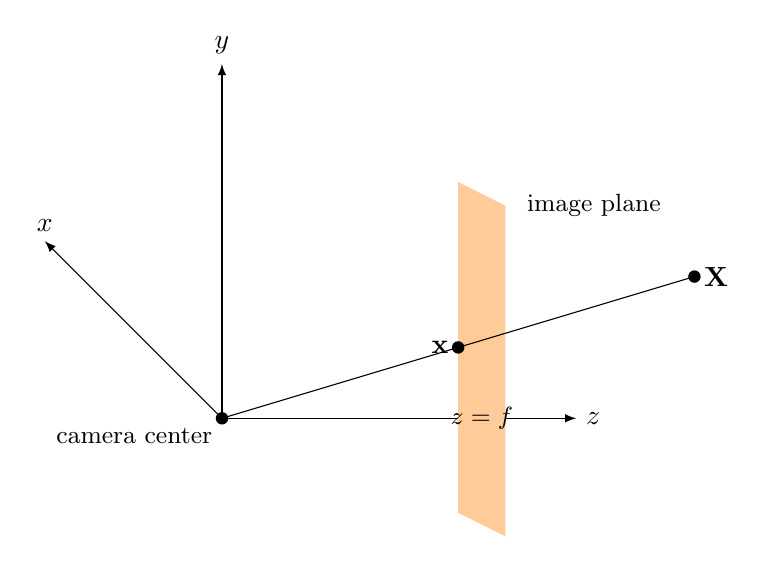
\begin{tikzpicture}[scale=1.5]

	% Define the coordinate system
	\draw[-latex] (0,0) -- (0,3) node[above] {$y$};
	\draw[-latex] (0,0) -- (3,0) node[right] {$z$};
	\draw[-latex] (0,0) -- (-1.5,1.5) node[above] {$x$};

	% Draw the image plane - adjusted angle and position
	\fill[orange!40] (2,-0.8) -- (2,2) -- (2.4,1.8) -- (2.4,-1) -- cycle;
	\node[right, font=\small] at (2.5,1.8) {image plane};
	\node[font=\small] at (2.2,0) {$z = f$};

	% Draw the camera center and label
	\fill (0,0) circle (1.5pt);
	\node[below left, font=\small] at (0,0) {camera center};

	% Draw the ray and points
	\draw (0,0) -- (4,1.2);
	\fill (2,0.6) circle (1.5pt) node[left] {$\mathbf{x}$};
	\fill (4,1.2) circle (1.5pt) node[right] {$\mathbf{X}$};

\end{tikzpicture}
\\ Consider the cross product:
\[
	\mathbf{x} \times (\mathbf{P} \mathbf{X}) = \mathbf{0}
\]
This equation enforces the condition that the 2D point \( \mathbf{x} \) lies on the projection of the 3D point \( \mathbf{X} \). The cross product between a point and a line is zero if and only if the point lies on the line, thus enforcing the geometric constraint.

% \subsection*{Cross Product Theory (CRSP)}
For two vectors \( \mathbf{a} = \begin{bmatrix} a_1 & a_2 & a_3 \end{bmatrix}^T \) and
\( \mathbf{b} = \begin{bmatrix} b_1 & b_2 & b_3 \end{bmatrix}^T \) in \( \mathbf{R}^3 \), their cross product is:
\[
	\mathbf{a} \times \mathbf{b} = \begin{vmatrix} \mathbf{i} & \mathbf{j} & \mathbf{k} \\ a_1 & a_2 & a_3 \\ b_1 & b_2 & b_3 \end{vmatrix}
\]


% \subsection*{ Formulating the System of Equations}

% For each corresponding 2D point \( \mathbf{x}_i \) and its projection \( \mathbf{P}_i \mathbf{X} \), we can write the constraint equation:
% \[
% \mathbf{x}_i \times (\mathbf{P}_i \mathbf{X}) = \mathbf{0}
% \]


Using the fact that the cross product should be zero

\[
	\mathbf{x} \times \mathbf{P} \mathbf{X} = 0
\]

\[
	\begin{bmatrix} x \\ y \\ 1 \end{bmatrix} \times \begin{bmatrix} \mathbf{p}_1^{\top} \mathbf{X} \\ \mathbf{p}_2^{\top} \mathbf{X} \\ \mathbf{p}_3^{\top} \mathbf{X} \end{bmatrix} = \begin{bmatrix} y \mathbf{p}_3^{\top} \mathbf{X} - \mathbf{p}_2^{\top} \mathbf{X} \\ \mathbf{p}_1^{\top} \mathbf{X} - x \mathbf{p}_3^{\top} \mathbf{X} \\ x \mathbf{p}_2^{\top} \mathbf{X} - y \mathbf{p}_1^{\top} \mathbf{X} \end{bmatrix} = \begin{bmatrix} 0 \\ 0 \\ 0 \end{bmatrix}
\]

Third line is a linear combination of the first and second lines.($x$ times the first line plus $y$ times the second line)
So one 2D to 3D point correspondence gives you 2 equations

\[
	\begin{bmatrix} y \mathbf{p}_3^{\top} \mathbf{X} - \mathbf{p}_2^{\top} \mathbf{X} \\ \mathbf{p}_1^{\top} \mathbf{X} - x \mathbf{p}_3^{\top} \mathbf{X} \end{bmatrix} = \begin{bmatrix} 0 \\ 0 \end{bmatrix}
\]

\[
	\begin{bmatrix} y \mathbf{p}_3^{\top} - \mathbf{p}_2^{\top} \\ \mathbf{p}_1^{\top} - x \mathbf{p}_3^{\top} \end{bmatrix} \mathbf{X} = \begin{bmatrix} 0 \\ 0 \end{bmatrix}
\]

\[
	A_i \mathbf{X} = 0
\]

Now we can make a system of linear equations (two lines for each 2D point correspondence)

For two views, we get two linear equations per correspondence, , we can form the following system of equations:

\[
	\begin{bmatrix}
		y \mathbf{p}_3^{\top} - \mathbf{p}_2^{\top}                \\
		\mathbf{p}_1^{\top} - x \mathbf{p}_3^{\top}                \\
		y' \mathbf{p}_3^{\prime \top} - \mathbf{p}_2^{\prime \top} \\
		\mathbf{p}_1^{\prime \top} - x' \mathbf{p}_3^{\prime \top}
	\end{bmatrix} \mathbf{X} = \begin{bmatrix} 0 \\ 0 \\ 0 \\ 0 \end{bmatrix}
\]

\[
	A \mathbf{X} = \mathbf{0}
\]
where \( A \) is a matrix that is constructed from the constraints given by the cross products. Each row of \( A \) corresponds to a linear equation derived from one cross product constraint.

\[
	A = \begin{bmatrix} \mathbf{a}_1^T \\ \mathbf{a}_2^T \\ \vdots \\ \mathbf{a}_{2n}^T \end{bmatrix}
	,
	\mathbf{X} = \begin{bmatrix} X \\ Y \\ Z \\ 1 \end{bmatrix}
\]


% \subsection*{4. Solving the System Using Singular Value Decomposition (SVD)}

To solve the system \( A \mathbf{X} = \mathbf{0} \), we use Singular Value Decomposition (SVD). The SVD decomposes the matrix \( A \) as:
\[
	A = U \Sigma V^T
\]
where \( U \) and \( V \) are orthogonal matrices, and \( \Sigma \) is a diagonal matrix containing the singular values of \( A \). The null space of \( A \) corresponds to the last column of \( V \), which is the solution to the homogeneous system.

Thus, the 3D point \( \mathbf{X} \) is the last column of \( V \):
\[
	\mathbf{X} = V_4
\]
The solution \( \mathbf{X} \) is normalized by dividing by the last element \( X_4 \):
\[
	\mathbf{X} = \frac{1}{X_4} \begin{bmatrix} X \\ Y \\ Z \end{bmatrix}
\]
This gives the real world 3D coordinates of user's head in non-homogeneous coordinates.



\begin{algorithm}[H]
	\caption{User's 3D Coordinates}
	\begin{algorithmic}[1]
		\Require user\_list (array of triplets: gesture, nose coordinates in frame-1, nose coordinates in frame-2)
		\Require fov1, fov2 (field of views of Cam-1 and Cam-2)
		\Require pos1, pos2 (real world positions of Cam-1 and Cam-2)
		\Require q1, q2 (quaternions for rotation of Cam-1 and Cam-2 from base unit vector in +x direction)
		\Ensure List of [(x,y,z), gesture] coordinates of each user with corresponding gesture
		\State result $\gets$ []
		\For{(gesture, nose1, nose2) in user\_list}
		\If{gesture is not None}
		\State Calculate dir1, direction vector from Cam-1 to user:
		\State Calculate nose coords from center of image:
		\State P.x $\gets$ nose1.x - frame\_width / 2
		\State P.y $\gets$ nose1.y - frame\_height / 2
		\State Find ratio between P and image dimensions:
		\State R.x $\gets$ P.x / (frame\_width / 2)
		\State R.y $\gets$ P.y / (frame\_height / 2)
		\State rot.z $\gets$ arctan(tan(fov1.horizontal / 2) * R.x)
		\State rot.y $\gets$ arctan(tan(fov1.vertical / 2) * R.y)
		\State q $\gets$ Quat::from\_euler(EulerRot::ZYX, rot.z, rot.y, 0.0)
		\State net\_rotation $\gets$ mul\_quat(q1, q)
		\State dir1 $\gets$ apply\_rotation(1i + 0j + 0k, net\_rotation)
		\State Calculate dir2 similarly using nose2 coordinates
		\State line1 $\gets$ Line::new(pos1, dir1)
		\State line2 $\gets$ Line::new(pos2, dir2)
		\State result.push((closest\_point\_between(line1, line2), gesture))
		\Else
		\State result.push(None)
		\EndIf
		\EndFor
		\State \Return result
	\end{algorithmic}
\end{algorithm}

\begin{figure}[!t]
	\centering
	\includegraphics[scale=1]{images/triangulation_concept.png} \\
	\caption{User’s direction vector from 2 camera system }
	\label{fig: User’s direction vector from 2 camera system }
\end{figure}


\subsection{Head Pose Estimation}
In our research, we utilize DirectMHP for accurate head pose estimation, providing Euler angles representing head orientation, for our main objective of determining the direction of the user's gaze to identify the device or object they are looking at within the environment

\begin{figure}[!t]
	\centering
	\includegraphics[scale=0.9]{images/euler_angles.png} \\
	\caption{Euler Angles for determining head pose }
	\label{fig: Euler Angles for determining head pose }
\end{figure}

To begin, we convert the Euler angles in Camera plane, $X_c$ into a quaternion representation $Q_c$. Quaternions offer advantages over Euler angles, such as avoiding gimbal lock and providing a more robust representation of rotations in three-dimensional space.

\tdplotsetmaincoords{70}{110}

\begin{figure}[h!]  % Use the figure environment for a caption
	\begin{center}
		\begin{tikzpicture}[tdplot_main_coords,
				vectorC/.style={-stealth,thick,red},
				vectorX/.style={-stealth,thick,green!50!black},
				dotted vectorC/.style={-stealth,thick,yellow!50!black,dotted},
				dotted vectorX/.style={-stealth,thick,blue,dotted},
				vectorXC/.style={-stealth, thick, magenta!80!black},
				axis/.style={-stealth,thick,black}]

			% Origin
			\coordinate (O) at (0,0,0);

			% Draw axes
			\draw[axis] (O) -- (4,0,0) node[anchor=north]{$x$};
			\draw[axis] (O) -- (0,4,0) node[anchor=west]{$y$};
			\draw[axis] (O) -- (0,0,4) node[anchor=south]{$z$};

			% Vector C
			\coordinate (C) at (2,1,3);
			\draw[vectorC] (O) -- (C) node[anchor=south]{$C$};

			% Vector C_o (dotted, coming out from C)
			\coordinate (Co) at (1,2,2.5);
			\draw[dotted vectorC] (C) -- (Co) node[anchor=south]{$C_o$};

			% Vector X
			\coordinate (X) at (1,4.5,1.5);
			\draw[vectorX] (O) -- (X) node[anchor=south]{$X$};

			% Vector D (dotted, coming out from X)
			\coordinate (D) at (2,5.5,3);
			\draw[dotted vectorX] (X) -- (D) node[anchor=south]{$D$};

			% vector X - C
			\draw[vectorXC] (X) -- (C) node[anchor=south]{};

		\end{tikzpicture}
		\caption{User's Head Orientation $D$ in world plane}  % Caption for the diagram
		\label{fig:3D_Orientations}  % Label for referencing in the document
	\end{center}
\end{figure}

Next, utilizing the head position coordinates $X$ and the primary camera coordinates $C$, we can calculate the direction of line of sight using quaternion multiplication as shown below:
\[
	D = Q \times \frac{(X - C)}{\| X - C \|}
\]

\subsection{Line of Sight}
By utilizing the head position coordinates $X$ as the anchor point and the transformed direction vector $D$, we determine the line of sight. This line represents the direction in which the individual is looking, providing valuable insight into their visual focus or intended actions.

Hence line of sight, L is given by:
\[
	L(t) = X + tD
\]

\subsection{Device Detection}
Devices are identified by checking which bounding boxes, each corresponding to a specific device, intersect with the line of sight. The device with the closest intersection is then selected as the target, upon which the action associated with the gesture is performed.
\begin{figure}[H]
	\begin{center}
		\begin{tikzpicture}
			%%% Edit the following coordinate to change the shape of your
			%%% cuboid

			%% Vanishing points for perspective handling
			\coordinate (P1) at (-7cm,1.5cm); % left vanishing point (To pick)
			\coordinate (P2) at (8cm,1.5cm); % right vanishing point (To pick)

			%% (A1) and (A2) defines the 2 central points of the cuboid
			\coordinate (A1) at (0em,0cm); % central top point (To pick)
			\coordinate (A2) at (0em,-2cm); % central bottom point (To pick)

			%% (A3) to (A8) are computed given a unique parameter (or 2) .8
			% You can vary .8 from 0 to 1 to change perspective on left side
			\coordinate (A3) at ($(P1)!.8!(A2)$); % To pick for perspective 
			\coordinate (A4) at ($(P1)!.8!(A1)$);

			% You can vary .8 from 0 to 1 to change perspective on right side
			\coordinate (A7) at ($(P2)!.7!(A2)$);
			\coordinate (A8) at ($(P2)!.7!(A1)$);

			%% Automatically compute the last 2 points with intersections
			\coordinate (A5) at
			(intersection cs: first line={(A8) -- (P1)},
			second line={(A4) -- (P2)});
			\coordinate (A6) at
			(intersection cs: first line={(A7) -- (P1)},
			second line={(A3) -- (P2)});

			%%% Draw the cuboid faces and lines as in the original code
			%% Possibly draw back faces
			\fill[gray!90] (A2) -- (A3) -- (A6) -- (A7) -- cycle; % face 6
			\node at (barycentric cs:A2=1,A3=1,A6=1,A7=1) {\tiny f6};

			\fill[gray!50] (A3) -- (A4) -- (A5) -- (A6) -- cycle; % face 3
			\node at (barycentric cs:A3=1,A4=1,A5=1,A6=1) {\tiny f3};

			\fill[gray!30] (A5) -- (A6) -- (A7) -- (A8) -- cycle; % face 4
			\node at (barycentric cs:A5=1,A6=1,A7=1,A8=1) {\tiny f4};

			\draw[thick,dashed] (A5) -- (A6);
			\draw[thick,dashed] (A3) -- (A6);
			\draw[thick,dashed] (A7) -- (A6);

			%% Possibly draw front faces
			\fill[gray!50,opacity=0.2] (A1) -- (A2) -- (A3) -- (A4) -- cycle; % f2
			\node at (barycentric cs:A1=1,A2=1,A3=1,A4=1) {\tiny f2};
			\fill[gray!90,opacity=0.2] (A1) -- (A4) -- (A5) -- (A8) -- cycle; % f5
			\node at (barycentric cs:A1=1,A4=1,A5=1,A8=1) {\tiny f5};

			%% Draw cuboid lines
			\draw[thick] (A1) -- (A2);
			\draw[thick] (A3) -- (A4);
			\draw[thick] (A7) -- (A8);
			\draw[thick] (A1) -- (A4);
			\draw[thick] (A1) -- (A8);
			\draw[thick] (A2) -- (A3);
			\draw[thick] (A2) -- (A7);
			\draw[thick] (A4) -- (A5);
			\draw[thick] (A8) -- (A5);

			% Draw points
			% \foreach \i in {1,2,...,8}
			% {
			%   \draw[fill=black] (A\i) circle (0.15em)
			%     node[above right] {\tiny \i};
			% }

			% Define point X outside of the cuboid (for example, at (4,4,5))
			\coordinate (X) at (4,3,4); % Example point X (outside the cuboid)

			% Draw line from point X to the cuboid (adjust coordinates if needed)
			\draw[thick, red] (X) -- (A3); % Line from X to A3 (example intersection)

			% Optionally, draw the intersection points or other visual indicators
			\draw[fill=blue] (X) circle (2pt) node[anchor=south] {\tiny X}; % Mark point X
		\end{tikzpicture}
	\end{center}
	\caption{LOS intersecting with bound box of device}
\end{figure}

\begin{algorithm}[H]
	\caption{Line of Sight (LOS) Calculation \& Identifying Target Device}
	\begin{algorithmic}[1]
		\Require array $A$ containing triplets of the \textit{Real world 3D coordinates of the users, the corresponding gesture and the Head Pose rotation}
		\Require $pos1$, real world position of Cam-1
		\Ensure array of pairs of the target device of each user, with the corresponding gesture
		\State $target\_devices \gets []$
		\For{$(position, gesture, pose)$ in $A$}
		\If{$gesture \neq None$}
		\State Calculate relative vector from the user to Cam-1: $rel \gets pos1 - position$
		\State Calculate direction vector of the user: $dir \gets apply\_rotation(pose, rel)$
		\State Construct line of sight: $los \gets Line::new(position, dir)$
		\State $candidates \gets$ get all devices whose bounding box intersect with $los$
		\State $closest\_device \gets None$
		\State $min\_distance \gets \infty$
		\For{$candidate$ in $candidates$}
		\State Check if device is in direction of $los$: $rel \gets candidate.position - los.anchor$
		\If{$rel \cdot los.dir \leq 0$}
		\State \textbf{continue}
		\EndIf
		\State $distance \gets rel.length()$
		\If{$distance < min\_distance$}
		\State $min\_distance \gets distance$
		\State $closest\_device \gets candidate$
		\EndIf
		\EndFor
		\State $target\_devices.push((closest\_device, gesture))$
		\Else
		\State $target\_devices.push(None)$
		\EndIf
		\EndFor
		\State \Return $target\_devices$
	\end{algorithmic}
\end{algorithm}

\subsection{Adding devices using rotating cameras}
Following calibration, we capture images from both cameras and mark corresponding points on each camera's image to identify the device's position, enabling the creation of a bounding box. For devices outside the cameras' current field of view, the cameras can be rotated to bring these devices into frame. Once visible, corresponding points on the bounding box can be marked and triangulated to establish precise positioning.
If the cameras' rotations are represented by rotation matrices $E_1$ and $E_2$, then:

New Rotation matrices of the cameras are,
\[
	R_1^\prime = E_1 \times R_1
\]
\[
	R_2^\prime = E_2 \times R_2
\]

The new extrinsic matrices of the cameras are,
\[
	M_{ext_1}^\prime =  \begin{bmatrix}
		R_1^\prime   & t_1 \\
		0_{1\times3} & 1
	\end{bmatrix}
\]
\[
	M_{ext_2}^\prime =  \begin{bmatrix}
		R_2^\prime   & t_2 \\
		0_{1\times3} & 1
	\end{bmatrix}
\]

where $t_1$ and $t_2$ are the translation matrices, which don't change due to rotation.

Now we can get the new projection matrices of the cameras as follow:
\[
	P_1^\prime = M_{int_1} \times M_{ext_1}
\]
\[
	P_2^\prime = M_{int_2} \times M_{int_2}
\]
